\documentclass[12pt,journal,draftcls,letterpaper,onecolumn]{elsarticle}
\usepackage{graphicx}
\usepackage{subfigure,multirow, algorithmic, algorithm}
\usepackage{setspace,tabularx,subfigure,epsfig,tabularx,amssymb,amsmath}

\newcommand{\algorithmicinput}{\textbf{Input}}
\newcommand{\algorithmicoutput}{\textbf{Output}}
\newcommand{\algorithmicvariable}{\textbf{Variables}}
\newcommand{\algorithmicmethod}{\textbf{Method}}
\newcommand{\algorithmicdescription}{\textbf{Description}}
\newcommand{\algorithmicbreak}{\textbf{break}}
\newcommand{\algorithmiccontinue}{\textbf{continue}}
\newcommand{\INPUT}{\item[{\algorithmicinput}]$\phantom{1}$}
\newcommand{\OUTPUT}{\item[\algorithmicoutput]$\phantom{1}$}
\newcommand{\VARIABLE}{\item[\algorithmicvariable]$\phantom{1}$\\}
\newcommand{\METHOD}{\item[\algorithmicmethod]$\phantom{1}$\\}
\newcommand{\DESCRIPTION}{\item[\algorithmicdescription]$\phantom{1}$\\}
\newcommand{\BREAK}{\STATE{\algorithmicbreak}}
\newcommand{\CONTINUE}{\STATE{\algorithmiccontinue}}


\begin{document}
%
% paper title
\title{Event Processing in Wireless Sensor Networks}

\maketitle


%\begin{abstract}

%\begin{itemize}
%
%  \item  \emph{Applications of event processing in Wireless Sensor Networks(WSNs)}
%  \item  \emph{Overview of event processing}
%  \item  \emph{Event processing in WSNs}
%  \item  \emph{Summary}
%\end{itemize}

%\end{abstract}


%\begin{keywords}
%Event, Event Message,
%\end{keywords}


\section{Applications of Event Processing in WSNs}

%event processing
\emph{Event processing}, as the classical topic in traditional
database areas, has been attracting more and more attention from the
research community of Wireless Sensor Networks (WSNs) \cite{332838},
\cite{345920}, \cite{Li03eventdetection},
\cite{DBLP:conf/vldb/AbadiML05}, \cite{dsware}. Considering the
previous studies of WSNs focus on continuous sensory data sampling
or in-network aggregating, this is an important and exciting change
in the WSN study. In comparison, event processing makes a WSN
\emph{smarter} and thus more efficient, as event processing realizes
a higher level data abstract.

Is changing WSNs from data collection to event processing necessary?
The answer is positive: The underlying motivation driving this
change is the need from the various applications, especially the
engineering applications \cite{990704}, \cite{sawant2004uba},
\cite{chen2006wws}, \cite{taniros04},
\cite{DBLP:journals/ijsnet/WangCLCXL09}, \cite{Low-Power05}. In
these engineering applications, the volume of sampled sensory data
for monitoring the status, detecting the abnormalities, or
predicating the results in manufacturing, etc., is tremendous
\cite{Li02detection}. Moreover, these engineering applications
usually have realtime requirements, long delay may cause the data
useless or disasters. However, routing back these large amount of
data to a central server within a short delay may be difficult or
impossible. Processing the data within a small number of nodes in
the network and recognize the event in realtime is thus the only
approach for the WSNs to be applied in these applications.


The follows present a number of example applications in two
representative engineering fields to illustrate the potential
benefits of event processing in WSNs. The first field is the
Intelligent Transportation Systems (ITS) and the second is the
Structure Health Monitoring (SHM) systems.

In the ITS field, researchers have attempted to apply WSNs in
transportation or vehicle monitoring. For instance, VigilNet
\cite{he2006vis} by He et al., the CarTel system
\cite{DBLP:conf/sensys/HullBZCGMSBM06} by Hull et al., the
TrafficView system \cite{1031487} and the PATH project
\cite{WEB:PATH} at UC Berkeley, etc. VigilNet focused on how to
efficiently and accurately track a moving vehicle in an hostile
environment. The authors of VigilNet proposed the time-driven system
design that enables the sensor nodes in a WSN to locally decide
their sensing and sleeping times based on the status of neighbors to
ensure the sensing coverage while observing the energy efficiency.

The above studies demonstrate the flexibility and applicability of
using WSNs in traffic monitoring. There are still lots of
application requirements that are not addressed. For example,
drivers may want the sensor nodes on the roadside to report the
possible collisions when they are driving on a road with
intersections; transportation management offices may want the WSN to
detect the road racing events, etc. All these need real-time event
detection, which cannot be served by a central data sink that is
collecting the traffic data. In addition, if these events could be
processed in the network instead of on the data sink (server), the
wireless network traffic would be greatly reduced. This, in turn,
helps the network to avoid wireless communication congestions.

Figure \ref{fig:application} shows a typical WSN setup in ITS. In
this figure, the left part shows the deployment of nodes with
magnetic sensors on a road of a cross-intersection and the right
part shows the network in the intersection. Suppose in this setup a
user specifies an event as a vehicle that is running in the wrong
direction at some lane (this example is in a left-hand traffic
country). As shown in this figure, the vehicle with $vid (Vehicle
ID) = 2$ is running in the wrong direction and node $S1$ is
currently monitoring it. This event requires the WSN to detect the
direction and the lane on which the vehicle is running.


\begin{figure}[ht]
\centering
\begin{minipage}{0.51\textwidth}
\includegraphics [width = 7cm]{realroad.eps}
\end{minipage}
\begin{minipage}{0.4\textwidth}
\includegraphics [width = 7cm]{application_scenario.eps}
\end{minipage}
\caption{Application scenario} \label{fig:application}
\end{figure}

However, node $s1$ itself cannot detect the direction with the
magnetic sensor. Figure \ref{fig:magnetic}a the magnetic sensory
data from a monitoring sensor node on the road of the previous
figure. In Figure \ref{fig:magnetic}a, the wave indicates that there
is a vehicle is approaching, running into, and then going away from
the sensor node. The height of the wave determined by the distance
between the sensor and the vehicle, which is used to detect the lane
of the vehicle. The span of the wave is determined by the velocity
and the length of the vehicle. Given this wave and suppose that each
sensor node can detect its own location, at least two such waves are
needed from sensor nodes at different locations to detect the
direction of a vehicle.


\begin{figure}[ht]
\centering
\includegraphics [width=15cm]{magnetic_data.eps}
\caption{Different sensor values} \label{fig:magnetic}
\end{figure}

In addition to the detection of direction, there are many elements
in traffic events need multiple sensor nodes to measure. For
instance, suppose in the above example the user needs the WSN to
broadcast the notification of the event to the vehicles that may
encounter the wrong vehicle within 5 seconds. In this example, the
WSN needs to detect the speed of the vehicles, but a sensor node
cannot tell the speed from the width of the wave in Figure
\ref{fig:magnetic}, as the wave width is determined by both the
velocity and the length of the vehicle.

Figure \ref{fig:magnetic} also shows that the data rate of a sensor
node should be high enough to detect the elements of an event.
Moreover, neither the absolute value of the wave trough nor the
height of the wave is constant in a WSN. The absolute value is
affected by the hardware, temperature and other environmental
factors. Under such a circumstance, it is either inefficient or
inaccurate to use a constant threshold in event detection.

Similarly, in the field of SHM, WSNs are being more and more
considered: In \cite{Krishna}, Krishnamurthy reported that the cost
of the installation of a wireless SHM system is less than half of
the wire-based counterpart. Another advantage of the WSN over
existing wired network is the higher spatial density of sensor
nodes. Compared with wire-based SHM systems, WSN permits a much
higher spatial density of sensors by replacing cables with wireless
communication. The total number of sensors deployed in a WSN can
reach hundreds or even thousands, which have the potential to
greatly enhance the quality of results that can be achieved. The
substantial benefits offered by WSN are mainly attributed to the low
cost wireless smart sensors.

The SHM systems based on WSNs are also in their initial stage.
Almost all SHM systems require high sensor sampling rates, large
storage size and high communication bandwidth. For example, to
capture the damage information from the sampled data from the
acceleration sensors, the sampling rate should be at least in the
kilo-Hz level. The data should be sent to the sink from time to
time, which needs the wireless communication device to transmit the
data in the Mbps level in a WSN with two or three nodes. The
bandwidth requirements on communication may be even much higher when
the network grows.

In-network data and event processing has been proposed to addressed
the problems in the WSN based SHM systems \cite{Mechitov},
\cite{pakzad:89}, \cite{DBLP:journals/ijsnet/WangCLCXL09},
\cite{Low-Power05}. Imagine when the sampled data are processed and
communicated within a small group of nodes or even within each node
itself, the network traffic would be significantly reduced. As the
network bandwidth is the bottleneck of these systems, this approach
is promising. The difficulty lies in the distributed algorithms to
detect the events of structure damage, which was previously
fulfilled by centralized algorithms. Researchers have proposed a set
of distributed algorithms, although there are still some problems in
accuracy and delay in these algorithms. In this chapter, we will not
discuss these algorithms but refer the interested readers to the
above studies, since the damage detection algorithms are not the
focus of this chapter. In the view of system architecture, the event
processing modules are on the top of the distributed algorithms
\cite{Messina}. Hence, when there are new algorithms for damage
detection, the event processing modules will be easily ported on top
of them.


However, event processing in WSNs is challenging, especially in the
above engineering applications. The major challenges are as follows.
(1) There is a conflict between the highly limited resources of WSNs
and the high requirements from engineering applications; (2)the
existing event processing techniques are not suitable for WSNs due
to their highly physical limited nature; (3) the WSNs are usually
unreliable due to frequent node or radio failures.

\section{Preliminaries}

\subsection{Terms}
%Event, Complex event, Composite event, Event message, Event %subscription,

\textbf{Event:} In the physical world, an \emph{event} is an
activity that occurred at some time and place. In computer science,
an event usually refers to a message that describes (records)
something happened. For instance, the appearance of a car on a road
is an event. A radio message that indicates this appearance of a car
in a WSN on the road is also called an event \cite{1483263}.

\textbf{Complex event:} A \emph{complex event} is an event that is
an abstraction of other events.  A complex event could only happen
if many of the other events happened \cite{1483263}. For example, an
event of car tire explosion is a complex event, which can be deduced
to has happened when a big "bang" was heard, the pressure of the
tire decrease suddenly, and the car becomes unstable.

\textbf{Composite event:} A composite event is a complex event in
which both the \emph{other events} and their relations are fixed
\cite{1483263}. For example, an event "two cars are running within a
distance of 5 meters for 5 minutes" is a composite event. This
composite event specifies the follows (1) the two car running events
occur at the same time; (2)their happening places are within a
5-meter distance and (3) the above relations of them last for 5
minutes.

\subsection{Previous Study}
\label{subsec:Previous Study}

With the terms defined, we now review the previous work on
high-level event processing techniques in both traditional computer
systems and WSNs. The review of event processing in traditional
systems is necessary, considering that the event processing study in
WSNs is relatively new and immature. Nonetheless, we omit the data
mining and pattern recognition techniques in event detection, since
they belong to the low-level data processing techniques. Under such
considerations, this section is partitioned into the following three
segments: (1) the event publish / subscribe paradigm for simple
event processing in traditional computer systems; (2) the event
patterns, rules, constraints, and event processing agent for complex
event processing in traditional computer systems; and (3) event
processing in WSNs.

The Event publish/subscribe (pub/sub) paradigm is the efficient and
effective way for event processing, especially in networking and
distributed systems \cite{DBLP:journals/csur/EugsterFGK03}. In this
event pub/sub, sers (Subscribers) can specify their interested
events (subscription) and will be notified if such events happen.
There is no direct connection between the subscriber and the
publisher. This is realized through decoupling of time, space, and
synchronization as follows: First, time decoupling, which means that
the publisher and subscriber may not start interaction at the same
time. The publisher can publish events even when the subscriber is
disconnected and vice versa, like off-line messages in the messenger
softwares. Second, space decoupling, which means that the pub/sub
parties interacts indirectly through event services. The publishers
do not know the number, the identity of the subscribers. Third,
synchronization decoupling, which enables the publisher and
subscriber to do  to in this scheme. Such decoupling makes the
pub/sub scheme much more flexible, in contrast to the point-to-point
or synchronous communications.

With the above pub/sub mechanisms, the event-driven systems are able
to receive the event subscription from users, detect the event using
the available data and event matching algorithms, and publish the
event to users. This is for simple events, as for complex events,
the event detection is a little different. We next study how the
complex events are detected using the event patterns, rules, and
constraints.

In a real world system, there are many events happening from time to
time. The ability to find some sets of events of interest from the
large number of events, is considered fundamental \cite{1483263}. A
template is needed so that the system is able to match the the set
of the events. The event pattern is thus defined as a template that
matches some specific sets of events interested. For example, the
red cars passed by the cross intersection \#1 yesterday. This
pattern specifies that all events of red car crossing the \#1
intersection are matched.


An event pattern rule is a reactive one that specifies the action to
be taken when the event pattern is matched \cite{1483263}
\cite{DBLP:conf/debs/SchieferRRS07}. An event rule has two parts:
(1) trigger: event pattern to match the event; and (2) action: the
event to be created when the trigger is activated.


The event processing agent (EPA) is the basic concept of complex
event processing. A class of EPAs is specified by an interface that
specifies the input/output actions, and behaviors of the event. The
three common EPAs are \emph{filter}, \emph{map}, and
\emph{constraint}. A filter is an agent that uses the event pattern
rules to pick out the interested events. A map is used to create new
(virtual) events based on the pattern recognition of the interested
events. An event constraint is different: it specifies the condition
that must be satisfied by the events. A constraint is a runtime
check, to ensure the system or the users behave normally. For
example, a constraint "never" can be used to specify that there are
no inconsistency among the requirements from users or to specify
that there are no conflicts between two events (e.g., running
eastward and westward of the same car simultaneously) of a complex
event.

Initial event detection in WSNs is realized via query processing
\cite{345920}, \cite{cougar}, \cite{tinydb}. For instance, Yao et
al. proposed a sensor database approach for the threshold-based
event detection in their Cougar system \cite{cougar}. Madden et al.
studied event triggers of queries in their acquisitional sensor
query processor, TinyDB \cite{tinydb}. The events are reported from
a query or a hardware device attached on a sensor node such as a
switch \cite{tinydb}. Hellerstein et al. extended the TinyDB query
engine to support much more sophisticated in-network data analysis
and event detection such as topographic mapping, and wavelet-based
compression \cite{Hellerstein03beyondaverage}. Moreover, Abadi et
al. proposed an in-network join scheme, REED, for joining sensor
data streams with static tables stored at the base station during
event detection \cite{DBLP:conf/vldb/AbadiML05}.

These query processing approach for event detection is not
applicable to traffic events, since the traffic events usually last
a long time whereas the query processor only get the snapshot data
or at most a short window of data.  Moreover, the attributes in
queries can be directly fetched or sampled by each sensor node. The
query processors do not consider the attributes that must be
measured by a few of sensor nodes, as mentioned in the examples of
the first section.

There are also middleware paradigms proposed for event detection in
WSNs \cite{1281625}, \cite{Li03eventdetection}, \cite{1101491}. The
EnviroTrack system \cite{1281625} uses a middleware component to
provide a convenient interface to application programmers for object
tracking. With EnviroTrack, a programmer
 needs to specify the functions for processing sensory data on
each sensor node, the aggregation function to process all sensory
data in a group that is tracking objects in the group. EnviroTrack
can invoke the user provided computation or actuation programs upon
object emergence.

DSWare \cite{Li03eventdetection} is another middleware system that
provides event detection services on sensor networks. The authors of
DSWare defined two types of events, atomic and compound events. An
atomic event is one that can be detected by one time sensor reading
(e.g., light $>$ 500). On the other hand, a compound event can only
be determined when the atomic events, which constitute the compound
event, are determined.

In the engineering applications, the above event processing
techniques may not be qualified. An event usually lasts a period of
time and its location may keep changing. For instance, an event ``a
vehicle changed lanes 4 times within 100 meters'' may require the
data from at least 5 nodes to detect the dynamic locations of each
vehicle. Even some events do not last such a long time, most still
cannot be detected by a single node. For example, a condition ``the
vehicle is running from south to north'' of an event needs at least
two sensor nodes at different locations to detect the vehicle
positions at two different times. Moreover, there are often strict
spatial-temporal constraints in an event, e.g.,``the vehicles
passing the third intersection within 20 minutes from now on''. This
requires the nodes strictly coordinate the timing and location of
their detected data, which is difficult for a distributed WSN.


In general, there are three significant open issues. First,
collaboration in event processing. These systems consider the
collaboration in in-network aggregation. Such in-network aggregation
only aggregates the same attribute or simply gather different
attributes from different nodes without considering their relations.
Second, these systems only support the attributes that can be
directly sampled from a sensing device but do not support an event
attribute that need several nodes to collaborate to detect. This
capability is especially important for a WSN in traffic event
processing, since there are many attributes such as speed, track,
etc. are not directly supported by the sensing devices. Third, the
direct event notification to moving nodes. Existing systems assume
the sink as the user to which the events should be routed. This is
not true for transportation and many event based applications.


\section{Event Processing in WSNs}

 This section describes the newly emerged
event processing techniques in WSNs. Their background applications
are mainly in ITS and SHM fields.

\subsection{System Model}
\label{sec:System Model}

%...............................................................
In event processing, there are two types of data, event subscription
and event notification. An event subscription describes what event
to detect and which destination nodes to notify when the event
happens. An event notification, on the other hand, inform the
destination nodes that the event is detected and provides the values
required in an event subscription. These two data structures are
similar to traditional event publish / subscription paradigms 
\cite{DBLP:journals/tocs/CarzanigaRW01}.

$Evt1$ gives the event subscription that requires a WSN to detect an
event of eastward moving vehicle on road \#1 and notify the event
elements such as lane, direction and speed of this vehicle to the
vehicles that are in a range of 1000 feet with this vehicle. The
notification message that is sent after the defined event is
detected should include the values of the elements.

$Evt1$: \emph{Report the lane, direction and speed of a eastward
moving vehicle on road \#1 to the vehicles that are within 1000 feet
away from this vehicle }.


%.............................................................

%
%\textbf{Node.} The architectures of the sensor and vehicle nodes are
%shown in Figure \ref{fig:sensor-vehicle-node}. As shown in this
%figure, a sensor node controls various sensing devices through the
%operating system and software drivers to sample the target
%characteristics. The patterns within these sampled data are
%recognized by the event processor in order to detect the
%user-interested events. In addition, the event processor may perform
%collaborative event detection when this node has received event
%notifications from its neighbors or may forward these notifications.
%
%\begin{figure}[ht]
%\centering
%\includegraphics [width=6cm] {sensor_node.eps}
%\caption{Event processing on a sensor node}
%\label{fig:sensor-vehicle-node}
%\end{figure}


The work flow on each node in a WSN is shown in Figure
\ref{fig:state_transition}. In this figure, the transition among the
six states is as follows. First, the nodes start the initialization
process to synchronize the time of themselves and set up the routes
for the later event notifications. The time synchronization is
needed for the nodes in collaborative event processing, since the
event elements that are processed on different nodes may have
temporal relations. The accuracy requirement to this time
synchronization is at the level of milliseconds, as the time unit of
vehicles is at the level of seconds. Then, each sensor node starts
the thread for processing the events.

\begin{figure}[ht]
\centering
\includegraphics [width=10cm]{state_transition.eps}
\caption{State transition in WSN event processing}
\label{fig:state_transition}
\end{figure}

The event registration state is to register the event subscriptions
injected by the users. The event decomposition, detection and
handling states are to process the event. Given a user-interested
event defined in the event subscription, a node should decompose the
event, if the event cannot be processed by the node itself. After
the event decomposition, a node may choose the sub-set of the data
that are needed in detecting the event. A group of nodes can then
collaboratively detect the event. When an event is detected, the
WSNs sometimes need to further handle the event, e.g., sending
control signals to the actuators of the systems, records the event
in the system log, etc. The details of the event composition,
detection, and handling are described next.


%-------------------------------------------------------------------------
\subsection {Event Registration and Notification: Pub/Sub}
%-------------------------------------------------------------------------
This section introduces a a pub/sub middleware, called PSWare, for
WSNs to register and notify the events. The current version of
PSWare supports the subscription and publish of composite events.
The architecture of PSWare is shown in Figure
\ref{fig:architecture}.


\begin{figure}[ht]
\centering
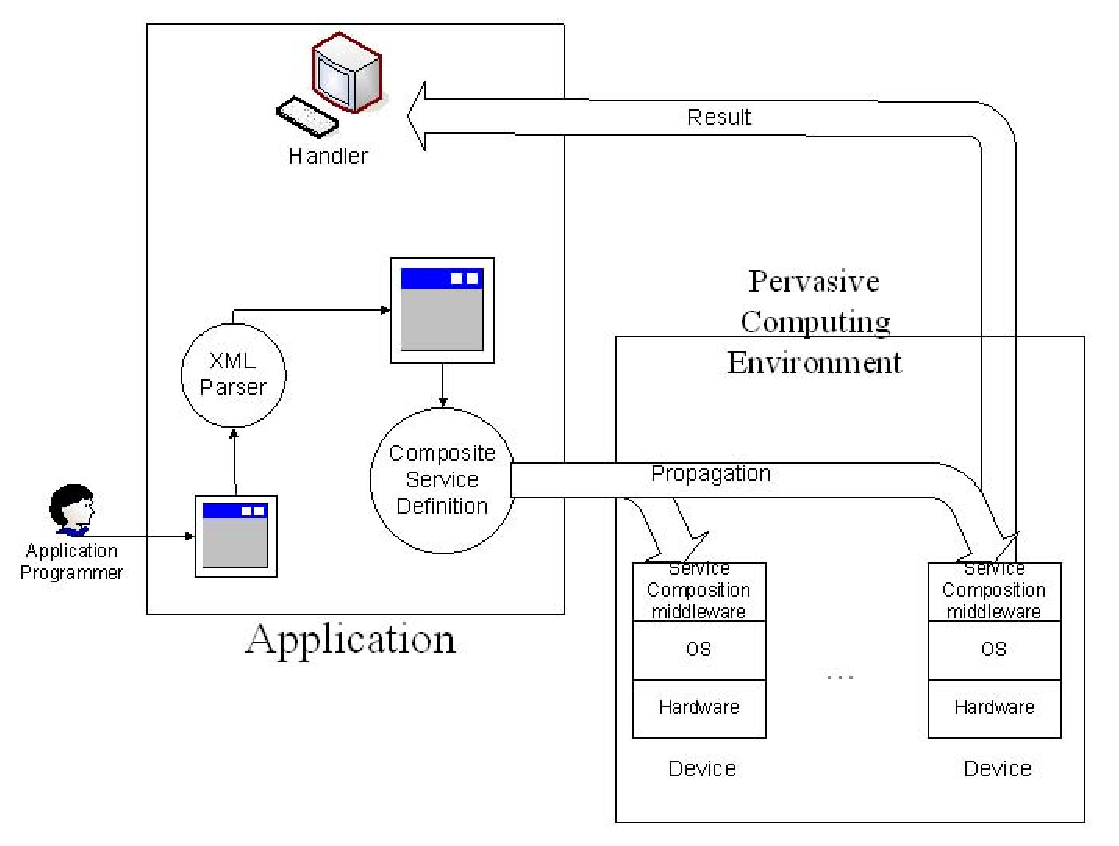
\includegraphics [width=15cm]{architecture.eps}
\caption{WSN pub/sub architecture} \label{fig:architecture}
\end{figure}


The major components of the pub/sub middleware are the compiler of
the Event Definition Language (EDL) and the VM (Virtual Machine)
runtime environment, and the event decomposer. EDL is a combination
of SQL and object-oriented language that defines the composite
events. The EDL compiler translates the high-level event definition
into low-level byte codes which can be further executed by
individual sensor nodes. The VM runtime environment runs the
compiled code of EDL so that the event decomposer can decompose the
event.

The workflow of the pub/sub middleware is as follows. First, event
registration: a user defines the events to be processed by a segment
of program using EDL. The compiler compiles this EDL program into
two parts as shown in Figure \ref{fig:bytecodes}. The first part is
the bytecodes which will later be disseminated and executed on
individual sensor nodes. The second part is the event receiving
module. This receiving module will interpret the data sent by the
sensor nodes and notify the application programmer whenever there
are incoming events. The bytecodes will be run on the VM and then be
processed by the event decomposer and the processor. Second, event
processing: the kernel event processing functions are performed by
the event decomposer and processor, which will be detailed in the
next two subsections. Third, event publishing: when there are events
detected, the middleware will publish the events by the receiving
module. In the following, we present the details of such subscribing
and publishing in this middleware.


\begin{figure}[ht]
\centering
\includegraphics [width=10cm]{compiler.eps}
\caption{Bytecodes} \label{fig:bytecodes}
\end{figure}


Specifically, the EDL program is compiled to the bytecodes before
they are disseminated to the sensor nodes. The bytecodes include the
program images for different functions. There are two types of
program images for the major event definition functions: the filter
and the event rule as shown in Figure \ref{fig:bytecodes}. The
concepts of the event filter and event rule are the same as those
defined in Section \ref{subsec:Previous Study}. Each of such program
image is a set of instructions that the VM can execute.


The VM runtime environment is based on Mate \cite{605407}. It uses
stack-based instructions to allow the execution of codes with
compact sizes. Due to the resource limitation of WSNs, this compact
size is significant to its applicability in real world applications.
The reason of choosing a VM-based runtime environment is that it is
more flexible in terms of interfacing with the EDL compiler and
introducing new modules. In addition, it is extensible to various
newly defined complex events. In contrast, those systems with fixed
event definitions and functions need to update programs to support
the new events.

%-------------------------------------------------------------------------

\subsection {Event Decomposition}

\label {sec:Event Decomposition}

With a composite event registered, the nodes in a WSN need to
decompose it to primitive events first so that they can process.
Usually, the event decomposition is done on each node. Although the
decomposition process can be done at a central node, the cost for
disseminating the decomposed sub-events is much more heavier than
that for decomposition. Before coming to the decomposition
algorithm, this section first presents the formulation of the events
that is used in event decomposition.

\subsubsection{Event Formulation}

An event is formulated as a 3-tuple, $E = \{F, P, C\}$, which is
valid within a time period $[t_s, t_e]$ and an area $S$. In this
3-tuple:
\begin{itemize}
\item $F$ is the \emph{field} set, which
describes the activity or property of the object(s) within the time
period $[t_s, t_e]$.
\item $P$ is the set of \emph{predicates}
on the fields.
\item $C$ is the set of \emph{connectors} for the predicates.
\end{itemize}

An item in the \emph{filed} set is an attribute of the object(s)
within the time period $[t_s, t_e]$ and area $S$. Suppose there are
$n$ field items $\{f_1, f_2, ...,f_n\}$, and the valid time period
of each item $f_i, (0 < i \leq n)$ is $[t_s(f_i), t_e(f_i)]$, then
$[t_s(f_i), t_e(f_i)] \subseteq [t_s, t_e]$. Moreover, all of these
items are valid only within the area $S$. In transportation
applications, the field set generally includes the following
attributes: vid, vehicle, speed, direction, lane, etc. Since an
event is valid within a time period and an area, the attribute can
also be a pattern, e.g., the track of a vehicle.

An item in the \emph{predicate} set gives the constraint on the
value of an attribute or on the relation of attributes in the
\emph{Field} set. Each predicate is a tuple \{$\alpha$, $o$,
$\upsilon$\}, where $\alpha$ is an attribute,
 \emph{o} is an operator on the attribute including$ <, >, =, \leq,
 \geq$. $\upsilon$ is the value operand for the operator.

The \emph{connector} set specifies the connection operators on
certain predicates to achieve more complex predicate logics. An item
in this set is also a tuple \{$\eta$, $c$, $\zeta$\}. $\eta$ and
$\zeta$ can be a {Connector} set or a single predicate. $\eta$ can
be an empty set. $c$ is an operator on $\eta$ and $\zeta$. The
possible operators include $\neg$ (not), $\bigvee$ (or), $\bigwedge$
(and).

We still take the previous event``a vehicle moving eastward on road
\#1'' as an example to illustrate the event formulation. In this
example, the valid time period of the event is the period when an
vehicle is moving eastward on the road. The field set of it is $F$ =
\{lane, direction, speed\}, The predicate set is \{ speed $>$ 0\,
direction $=$ eastward \}. The connector set is \{\textbf{and}\}.

\subsubsection{Three Level Sub-Events}

With the above formulation of attributes and predicates in an event,
an sub-event of this event is formulated as the attributes or parts
of the attributes, and the predicates within the valid time period
and area of this event. There are three levels of sub-events:
multiple attribute sub-event (MS), single attribute sub-event (SS)
and partial attribute sub-event(PS). In SS and PS, the event that
can be processed by a single node (without the data from others) is
called a primitive event.

The reason for dividing these three levels of sub-events is as
follows. An MS carries the relationships between the attributes. For
instance, an MS of the event ``a vehicle of speed $>$ 100 and
direction $=$ eastward at intersection 2" can be ``speed $>$ 100 and
direction $=$ eastward''. The single attribute sub-event is for the
attributes that can be detected by a single node. For example, the
attribute \emph{vid} can be constructed to an SS. The partial
attribute sub-event is for the attributes that should be detected by
several nodes. For instance, the attribute \emph{speed} should have
two PSs, since it needs two motes to detect.

A single event can have infinite number of sub-events at each level
(MS, SS, PS), when two or more sub-events overlap. Overlapping
refers to the state that the sub-events have the same attribute
within overlapping time periods and areas. Due to the resource
limitation of WSNs, it is desirable to find the set of sub-events at
each level with the minimum overlap.

\subsubsection{Event Partition}

All of the non-overlapped sub-events of an event constitute a
partition of the event. Apparently, there will be no resource waste
in processing a partition of an event. Algorithm \ref{alg:Partition}
shows how to partition an event to the three levels of sub-events.

\begin{algorithm} [ht]
\caption{Event partition} \label{alg:Partition}
\begin{algorithmic}
\INPUT $E = \{F, P, C\}$;
\OUTPUT A set of $n$ sub-events: $\{E_s\}, 0 < s \leq n$; \STATE /*
first step */ \STATE $n = 0$, $i = 1$; \WHILE{$|E.F| > 0$}
    \STATE $F_i = closure(E.F.f_i)$; //\emph{subset of attriutes that are connected with $E.F.f_i$ by connectors}
    \STATE $E_i = \{F_i, \{P_i\}, C\}$;
    \STATE $E.F = E.F - F_i$;
    \STATE $n = n + 1$, $i = i + 1$;
\ENDWHILE \STATE /* second step */
%\STATE $O''_1, O''_2$: recheck if there are queries in the waiting
%lists that can be satisfied now and append them to the query queue
%of $O'_1$ and $O'_2$.
%\STATE /* the following will partition the sub-events which include more than one attributes to single attribute sub-events */
\FOR{each sub-event $E_i$}
   \FOR{$j = 1$ to $|E_i.F|$}
       \IF {$|E_i.F| > 1$ or $E_i.F$ is not detectable by a single node}
           \STATE $E_{ij} = \{\{E_i.F.f_j\}, \phi, \phi \}$ // using rules given in the system catalog
           \STATE $n = n + 1$;
       \ELSE
           \STATE $E_{ij} = E_i $;
           \STATE remove $E_i$
       \ENDIF
   \ENDFOR
\ENDFOR

\end{algorithmic}
\end{algorithm}

\textbf{Property 1:} \emph{The semantics of the original event is
the same as that of the sub-events from Algorithm
\ref{alg:Partition} }

\textbf{Proof:} First,  Algorithm \ref{alg:Partition} ensures that
each sub-event in the first level preserves the dependencies between
the attributes in it, since the first step in the algorithm does not
remove the relations between the attributes. When the first level
sub-events are decomposed to single attribute sub-events, the valid
time period and location of each attribute are not changed.
Collectively, the two level sub-events from Algorithm
\ref{alg:Partition} preserve the relations and temporal-spatial
properties of the original event. Moreover, there is no attribute
lost during the decomposition. Therefore, the semantics of the
decomposed sub-events is the same as that of the original event.
$\Box$

Finally, we show an example of the sub-events and their relation
derived from the event decomposition. The sub-events are built up
into a tree, as shown in Figure \ref{fig:Event tree}.

\begin{figure}[ht]
\centering
\includegraphics [width=10cm]{event_tree_g.eps}
\caption{Tree of the sub-events of Evt1} \label{fig:Event tree}
\end{figure}

In Figure \ref{fig:Event tree}, each level of the tree describes a
level of sub-events. The relation between the sub-events are
connected either by the branch lines in the tree or by the arrows.
The branch line between two sub-events denote that the lower level
sub-event provides the input to the higher level one. The arrow
between the sub-events indicate the spatial-temporal relations
between the sub-events. In this figure, the arrow between
\emph{vehicle} and other sub-events specifies that the other
sub-events should be detected after this \emph{vehicle} sub-event
within a delay of $Th$. Next, we show how to detect the sub-events
whose relations are given in such a tree.

\subsection{Collaborative Event Detection}

\label{sec:Event Processing}


Given the decomposed sub-events of an event subscription, the event
processor constructs an \emph{event detection tree} in the reverse
manner to the event decomposition. The tree gives an event detection
plan. Then the nodes dynamically collaborate to detect the
sub-events according to this event detection plan.

The event detection plan given by the tree is similar to that of
traditional databases in that both use operators as the nodes of the
tree to describe the plan. However, there are three major
differences between an event detection plan (EP) and a query
evaluation plan (QP) are as follows. (1) An EP defines the timing,
lasting periods and locations of each operator so that the relations
between the attributes are reserved in event detection, whereas a QP
does not. (2) The operators in an EP are on the sub-events with
partial or single attributes of an event. However, the operator of
QP is on a tuple with all attributes in a table. Apparently, such
operator in an EP is more suitable for the energy efficiency in
event detection. (3) An EP specifies the time series between two
operators when the sub-events that these two operators detect have
strict temporal order. In contrast, a traditional QP does not have.

\subsubsection{Event Operator}

Each sub-event resulted from the event decomposition is to be
processed by an \emph{event operator}. An event operator is a
function unit in event processing. There are totally six types of
general event operators as follows: \emph{sensing},
\emph{extracting}, \emph{filtering}, \emph{aggregating},
\emph{assembling}, \emph{receiving}, and \emph{notifying}.

A \emph{sensing} operator is to sample one of the current physical
characteristics of a target using a sensing device on a sensor node.
Hence, there are usually a series of different sensing operators for
sampling the data from the different sensing devices. A sensing
operator is executed when a user is interested in some events on a
target that can be inferred from the sensory data of the target.
Usually, a sensing operator runs periodically, since the target
keeps changing but the operator can get one snapshot of the target
only. The cycle of such periodical sensing should be set shorter
than the target changing rate and longer than the device delay, if
possible.

An \emph{extracting} operator processes the sensory data and
extracts the physical characteristics of the target. For instance,
an extracting operator can be used to recognize the approaching of a
vehicle. A subsequent issue of such extracting operators is the
operator update. Since the extracting operator is much more complex
than the usual operators such as sensing, the implementation of an
extracting operator may need to be updated from time to time, when
there are new patterns needed to be detected. Such operator update
operation can be done by using a dynamic link module, which can be
updated via wireless communication\cite{1067188}, \cite{1160178}.

A \emph{filtering} operator removes the unwanted data during event
processing and finally checks whether the user registered event
occurs when all data are ready. The output of the extracting
operators or a sub-event as an attribute in an filtering operator.
For instance, the filtering operator $snake(direction)>0.04$ checks
whether a vehicle follows a snake pattern: keeps changing lanes in a
short distance (Suppose that 0.04 is defined as 4 times lane
changing within the 100 meter). The code of the extracting operator
$snake$ is defined and maintained by the server of a WSN.

An \emph{aggregating} operator summarizes the data in several events
and generates one event that describes the summary of these events.
Aggregation is commonly used in traditional databases for users to
get statistical information of the data. The communication traffic
is much lighter when only one event notification is sent out after
this aggregation than that without aggregation.

An \emph{assembling} operator performs the following operations on
sub-events: first, it picks out the data in the sub-events; then, it
packs the needed data to the data field of a new event. Since a
sensor node may not be able to get all sub-events ready at one time
or sometimes cannot get all of the sub-events of an event itself,
this assembling operator is necessary to produce the partial
results. Note that this operator
 processes different types of data or attributes, which is the
key difference from the aggregating operator.

A \emph{receiving} operator is for a sensor node to receive the
notifications of sub-events or events from its neighbors. After
receiving, the sensor node can use the information in these
notifications and its own information to further process or update
the values of the attributes in the notifications.

Finally, a \emph{notifying} operator is to send the message that
indicates some sub-events of the event are detected. This operator
is different from the event notifying operation in event handling in
that the former is for sub-event notifications and collaboration but
the latter is for the notification of the entire event. Nonetheless,
they can use the same modules for communication. The notification
message of a sub-event is a set of fields and their values. We add a
tag: \{$timestamp$, $location$\} to a notification message to
indicate when and where this event was detected.


\subsubsection{Event Detection Tree}

With the above operators, we present the event detection tree that
provides the event detection plan. The follows use two examples to
show such a tree for both single event and multiple events.

Suppose the registered event is $Evt1$ (see Section \ref{sec:System
Model}). First, the nodes on Road \#1 in partitions $Evt1$ to a tree
of three levels of sub-events, each of which is to be processed by
an operator. Then, an evaluation tree with the corresponding
operators is constructed by replacing operators to the sub-event
tree. Figure \ref{fig:Event detection tree} shows the detection tree
of $Evt1$. In Figure \ref{fig:Event detection tree}, the operators
to process the sub-events are connected in accordance with the
relation between the sub-events. The triangular operator denotes the
extracting operator, e.g., vehicle, speed, etc.

In Figure \ref{fig:Event detection tree}, the detection tree use a
trigger line from the operator \emph{vehicle} to denote the temporal
relation between the sub-events. The trigger signal from the
operator \emph{vehicle} starts an operator at the end of each arrow,
when this \emph{vehicle} operator detects the appearance of a
vehicle. As a result, the triggered operators are synchronized with
the vehicle appearance. The timing of the trigger is regulated as $T
< Th$, which specifies that the delay of starting the triggered
operators should be less than $Th$. The location and timestamp
($T_1$) information from the sensing operator are the location of
the node and the time the node detects the vehicle. The timestamp
The constraint between the timestamp from a neighbor, $T_0$, and
$T_1$ is for the correctness of event detection, since the
communication or timing failures are not rare in a WSN.

\begin{figure}[ht]
\centering
\includegraphics [width=8cm]{evaluation_tree_g.eps}
\caption{Global event detection tree of Evt1} \label{fig:Event
detection tree}
\end{figure}

Figure \ref{fig:Event detection tree} only gives the global event
detection plan for $Evt1$. For a group of sensor nodes to
collaboratively process a event, each sensor node should use a local
event detection tree and the local detection trees of the group
constitute the whole detection plan of the event. This mission on
each sensor node is completed in two steps: First, decides what
sub-events it will process. Second, creates a view of a local
detection tree on the exiting global event detection tree with
regard to the sub-events to be processed by this node.

As described in Section \ref{sec:Event Decomposition}, each sensor
node is aware of all of the sub-events of $Evt1$ since it performs
the event decomposition using the rules in the system catalog. Then
it decides what sub-events to process itself following the three
rules listed below. Note that in other kinds of applications, these
three rules may need to be extended , since the event subscriptions
may have special requirements on the quality of services, which will
affect the standard of choose sub-events for processing.
\begin{enumerate} \itemsep -2pt
   \item Process the processable sub-events that must be processed on
the sensor node.
   \item Process the remaining unprocessed sub-events that use the sub-events of
neighbors as inputs, if available resource allows, otherwise,
forward the received sub-events to its neighbors.
   \item Process the remaining unprocessed sub-events after that use the sub-events if available
resource allows.
 \end{enumerate}

With the sub-events chosen, a sensor node creates a view of
detection tree based on the global event detection tree. The
algorithm for creating a view of local event detection tree
following these rules is shown in Algorithm \ref{alg:Collaborative}.
This algorithm creates a view of the local detection tree, which is
composed of a new notification operator, a new assembling operator,
and operators marked as active in the global tree. The new
notification operator is for sub-event notification and the new
assembling operator is for wrapping up the outputs from the other
operators in the tree view. The previous notification and assembling
operator are not used in the view in order to keep the relations of
the sub-events in the event.

\begin{algorithm} [ht]
\caption{Create a view of local detection tree}
\label{alg:Collaborative}
\begin{algorithmic}
\INPUT Global evlauation tree $T$, received notifications $\{S_k\}$;
\OUTPUT A view of local event detection tree VT
    \STATE $\{E_s\}$ = sub-events should be processed on this node according to the three rules
    \STATE VT.root = new(notifyingOp)
    \STATE curNode = new(assemblingOp)
    \STATE Add curNode as a child to VT.root
    \STATE $h = 1$ // h: the height of an operator in $T$, $h$ of the root is 0.
    \WHILE{$\{E_s\} \neq \phi$}
       \FOR{each non-receiving operator node $T.n_i$ at height $h$ of T \textbf{and} $T.n_i.E_i \in \{E_s\}$}
            \STATE Add $T.n_i$ as a child of curNode
            \STATE $T.n_i.active = true$
            \STATE $\{E_s\} = \{E_s\} - T.n_i.E_i$
            \STATE Recursively mark each $T.n_j$ in the sub-tree of $T.n_i$ as active; and $\{E_s\} = \{E_s\} -
            T.n_j.E_j$
       \ENDFOR
       \STATE $h = h + 1$
    \ENDWHILE
    \FOR{each receiving operator node $T.n_k$ with output $S_k$ \textbf{and} $
    T.n_k.active$ is false}
        \STATE Add $T.n_k$ as a child of curNode
        \STATE $T.n_k.active = true$
    \ENDFOR
\end{algorithmic}
\end{algorithm}

We now demonstrate how this algorithm creates the view of a local
detection plan tree on a group of sensor nodes, which are processing
$Evt1$. Suppose $Evt1$ is registered on three sensor nodes: x, y,
and z that are deployed in the same eastward line on a road and a
vehicle is driving approaching x first.

Node x first detects the vehicle and starts to create the view for
the event evaluation. It finds that it can detect the $vid$ and
$lane$. Node x is not able to calculate the $speed$ and $location$,
since it is the first sensor node to detect this vehicle and did not
receive the needed information on this vehicle from other sensor
nodes. The view of this detection plan is shown in Figure
\ref{fig:View of detection tree on node x}. Note that the operator
\emph{vehicle} is not in this view, since it has already activated
the operators before creating the view and will no longer run in
this view.

\begin{figure}[ht]
\centering
\includegraphics [width=9cm]{evaluation_tree_x.eps}
\caption{The view of detection tree on x} \label{fig:View of
detection tree on node x}
\end{figure}

Node y receives the sub-event notification from node x but it will
not start algorithm \ref{alg:Collaborative} immediately. It buffers
the notification and waits until the \emph{vehicle} operator
activates the algorithm, i.e., it detects the vehicle. The event
detection plan on node y after vehicle triggering is shown in Figure
\ref{fig:Complete event detection tree}.

\begin{figure}[ht]
\centering
\includegraphics [width=9cm]{evaluation_tree_y.eps}
\caption{The view of detection tree on y} \label{fig:Complete event
detection tree}
\end{figure}

Whether node $z$ participates in this collaborative processing is
determined by the user requirements. If the user of $Evt1$ specifies
that $Evt1$ only needs to be detected once, then node z will merely
forward the event notification from node y towards the destination
nodes; Otherwise, node z forwards the notification from y and
processes the event when it finds the same vehicle use the event
notification from y as an input and node z may send a new
notification if the attribute values of the event changed.

Note that the detection plan on a sensor node is not fixed due to
following dynamics: (1) the data of events (vehicle is moving), (2)
wireless communication (delay, failure, etc.), and sensor nodes
(failure, available resources) on roads. In the above example, if
node x was unable to detect the sub-event of $vid$, due to the
failure of its sensing device or node y did not receive the
sub-event from node $x$, then node $y$ uses the same view as that of
node $x$. Consequently, the event processor is able to reliably deal
with complex events, regardless of the hardware and topology
dynamics.


%Multi-event-node detection tree.
Next we use another example to illustrate how to detect multiple
events with the event detection tree. Suppose there are two events,
$Evt1$ (Section \ref{sec:System Model}) and $Evt2$ as shown below.

 $Evt2$: \emph{Report the location, vid and speed of a vehicle whose
speed $>$ 100 mph OR  who changed lane 4 times within 120 feet to
the police vehicles within 10 miles}.

Suppose the distance between two sensor nodes is 25 feet in a WSN.
Then this event needs at least 5 location consecutive sensor nodes
to collaboratively process. In this WSN, the event processor on each
sensor node first constructs the global detection plan based on the
sub-events, as shown in Figure \ref{fig:Multiple event detection
tree}. Since the event processing scheme connects the different
inputs and outputs to the tree sensor nodes (operators), the common
sub-events among the two events, e.g., $vid$ can share the same
operators. Moreover, the scheme adds a virtual operator as the root
of the tree. The children of this virtual operator are the
notification operators for the two events. In Figure
\ref{fig:Multiple event detection tree}, the extracting operator of
snake requires the inputs from at least five sensor nodes. The snake
value is calculated as lane changing times within a segment of road
divided by the length of this segment.

\begin{figure}[ht]
\centering
\includegraphics [width=9cm]{multiple_evaluation_tree_g.eps}
\caption{Detection tree of multi-events} \label{fig:Multiple event
detection tree}
\end{figure}

Suppose there are five nodes, nodes 1-5, within 120 feet on a road.
The view of the local detection tree on node 1 is the same as that
of node x in the previous example in Figure \ref{fig:View of
detection tree on node x}. The reason is that the sub-events in the
tree are all that node 1 can detect, as the first node to detect a
vehicle. The views of nodes 2-5 are similar to the tree in Figure
\ref{fig:Multiple event detection tree}, since the process of
creating the view on each of them is the same as that of node y.

\subsection{Performance Analysis}
\label{subsec:Performance Analysis}

This section analyzes the event processing cost including both the
time cost and energy cost of the above collaborative event
processing technique. These costs are critical for the practicalness
of an event processing system that involves the deployment of real
sensor nodes on roads.

As illustrated in the previous section, the event evaluation time on
each node is the total time of executing the event operators,
including the time for receiving and transmitting the values of
sub-events or events. Considering this, the time cost of each node
in processing an event can be modeled in Equation \ref{eq:time
cost}. In this equation, $n$ is the total number of operators, $T_i$
is the time cost of each operator. $m$ is the number of parallel
operator groups, within which the operators can run in parallel.
$P_j$ is overlapping time of the operators in each group. For
instance, some sensing operators of different types can run in
parallel.

\begin{equation} \label{eq:time cost}
T = \sum^{n}_{i = 1} T_i - \sum^{m}_{j = 1} P_j
\end{equation}

Suppose a sleeping scheduling protocol enables a node to sleep after
it finishes event processing. As sleeping consumes the lowest
energy, we omit the energy cost of sleeping and calculate the energy
cost of each node in Equation \ref{eq:energy cost}. In Equation
\ref{eq:energy cost}, $k$ is the number of non-communication
operators, $E_i$ is the energy consumption of a non-communication
operator. $E_r$ and $E_t$ are the energy cost of receiving and
transmitting a packet, respectively.

\begin{equation} \label{eq:energy cost}
E = \sum^{k}_{i = 0} E_i + E_r + E_t
\end{equation}

The energy cost of a node that forwards data to the sink for event
detection is estimated in Equation \ref{eq:forward cost}. In this
equation, $E_p$ is the energy consumption in computation. $h$ is the
height of the node, $h$ = 0 for a leaf node. $C$ is the average
number of nodes that transmit data to an internal node for
forwarding at each hop. In comparison, the collaborative in-network
event processing scheme confines the communication within one hop
neighbors and thus can significantly reduce the energy cost as well
as the communication delay.

\begin{equation} \label{eq:forward cost}
E = E_p + \sum^{h}_{i = 1} i \times C(E_r + E_t) + E_t
\end{equation}


\subsection{Event Handling} \label{sec:Event Handling}

When an event is detected, a WSN should handle the event. This event
handling operation differs in the various applications. Here we give
an example in ITS to illustrate the logic of event handling in an
event processor.


\textbf{Event Notification.} To route the notification message to
the destination nodes specified in the event subscription, a
multicast routing protocol is needed. In general, a geographic
routing protocol can be used to forward the notification messages.
This protocol works as follows: when a node receives a notification
message, it compares the location of the source node and the
destination nodes. If this node is closer to the destination nodes,
it will forward the message, otherwise, it will discard the message.
There are quite a few geographic routing protocols that can be used
for this purpose.

\textbf{Event-Driven Actuation.} There are some applications that
need the sensor nodes to actuate the vehicles in transportation
systems. For example, there are often event subscriptions involve
intersections such as ``report speed, direction and lane of a
vehicle 20cm away from any intersection to the vehicles within 40cm
distance to this vehicle''. These kind of event subscriptions need
the vehicles including sender and destined receivers to actuate in
accordance to the event notification.

To alleviate the burden of a programmer in building up the programs
for such event-driven actuation, a set of distributed actuation
protocols can be used for the common actuation applications. Take
the ITS filed as an example, the protocols on each vehicle node
control the vehicle according to the transportation rules and the
road map, upon an event. The following is a command in the protocol:
\emph{Upon event eid = x, do collision-avoidance}.

The follows show an example of such actuation on a WSN-based ITS
testbed. Figure \ref{fig:Event handling} shows that two model cars
are communicating and controlling themselves to avoid collisions at
a T-intersection road. In this figure, the model car turning left
was yielding at the entrance of the intersection. The actuation
modules installed on the MICAz motes in that are controlling the
model cars on the model transportation testbed.


\begin{figure}[ht]
\centering
\includegraphics [width=10cm]{yield.eps}
\caption{Event handling}\label{fig:Event handling}
\end{figure}

\subsection{Support event processing in SHM systems}

The above sections mainly present event processing in the background
of ITS. We now discuss the event processing problems in SHM: In a
WSN-based SHM system, an array of sensors, usually accelerometers
and strain gauges, are deployed on the structure to be monitored to
periodically monitor its responses to ambient or forced excitation.
From these measurements, SHM algorithms are carried out to extract
damage-sensitive features and compares these features with reference
ones which are obtained when the structure is healthy.  From the
change of the features, information about damage occurrence, damage
location and even the severity of damage can be obtained. SHM
algorithms usually can be classified as four levels of damage
assessment:

\begin{itemize}
    \item     Level 1 (detection): Determination that damage is present in the structure.
    \item     Level 2 (localization): Level 1 plus determination of the geometric location of the damage.
    \item     Level 3 (quantification): Level 2 plus quantification of the severity of the damage.
    \item     Level 4 (prediction): Level 3 plus the prediction of the structure life, damage .
\end{itemize}

The levels 1 and 3 are mainly the tasks for the data analysis
algorithms \cite{1475888}, \cite{1507526}. The other two levels are
in effect the function of event detection and notification. With the
event processing system presented in the previous sections, the
users can input their requirements for monitoring such as accuracy,
frequency, delay, etc. The event processing system runs the data
analysis algorithms to detect the damage, report the damage location
and predict the structure life.

%-------------------------------------------------------------------------

\section{Summary}

This chapter first presents the applications that call for
in-network event processing in WSNs, demonstrates the benefits of
event processing and analyzes the feasibility of such event
processing. It reviews the event processing techniques in both
traditional database areas and WSNs. Finally this chapter describes
an event processing paradigm with a pub/sub middleware and a
collaborative event processor for WSNs. Overall, the techniques are
described in detail and the performance benefits of event processing
in WSNs are discussed.


\bibliographystyle{abbrv}
\bibliography{references}

\end{document}


%
%
%%\hfill mds
%%
%%\hfill August 10, 2009
%
%\subsection{Subsection Heading Here}
%Subsection text here.
%
%% needed in second column of first page if using \pubid
%%\pubidadjcol
%
%\subsubsection{Subsubsection Heading Here}
%Subsubsection text here.
%
%
%
%\section{Conclusion}
%The conclusion goes here.
%
%\appendices
%\section{Proof of the First Zonklar Equation}
%Appendix one text goes here.
%
%\section{}
%Appendix two text goes here.
%
%% use section* for acknowledgement
%%\section*{Acknowledgment}
%%% optional entry into table of contents (if used)
%%%\addcontentsline{toc}{section}{Acknowledgment}
%%The authors would like to thank... This work was supported by the
%IEEE.
